% Created 2018-04-18 Wed 17:15
% Intended LaTeX compiler: pdflatex
\documentclass[11pt]{article}
\usepackage[utf8]{inputenc}
\usepackage[T1]{fontenc}
\usepackage{graphicx}
\usepackage{grffile}
\usepackage{longtable}
\usepackage{wrapfig}
\usepackage{rotating}
\usepackage[normalem]{ulem}
\usepackage{amsmath}
\usepackage{textcomp}
\usepackage{amssymb}
\usepackage{capt-of}
\usepackage{hyperref}
\author{Peter Polidoro}
\date{\today}
\title{modular\_device\_base\_3x2}
\hypersetup{
 pdfauthor={Peter Polidoro},
 pdftitle={modular\_device\_base\_3x2},
 pdfkeywords={},
 pdfsubject={},
 pdfcreator={Emacs 27.0.50 (Org mode 9.1.9)},
 pdflang={English}}
\begin{document}

\maketitle
\tableofcontents


\section{Repository Information}
\label{sec:org53f9fb2}
\begin{description}
\item[{Title}] modular\_device\_base\_3x2
\item[{Author}] Peter Polidoro
\item[{Email}] peterpolidoro@gmail.com
\item[{License}] Open-Source Hardware
\end{description}

\section{Schematic}
\label{sec:org4149065}

\href{./schematic/modular\_device\_base\_3x2.pdf}{modular\_device\_base\_3x2.pdf}


\begin{center}
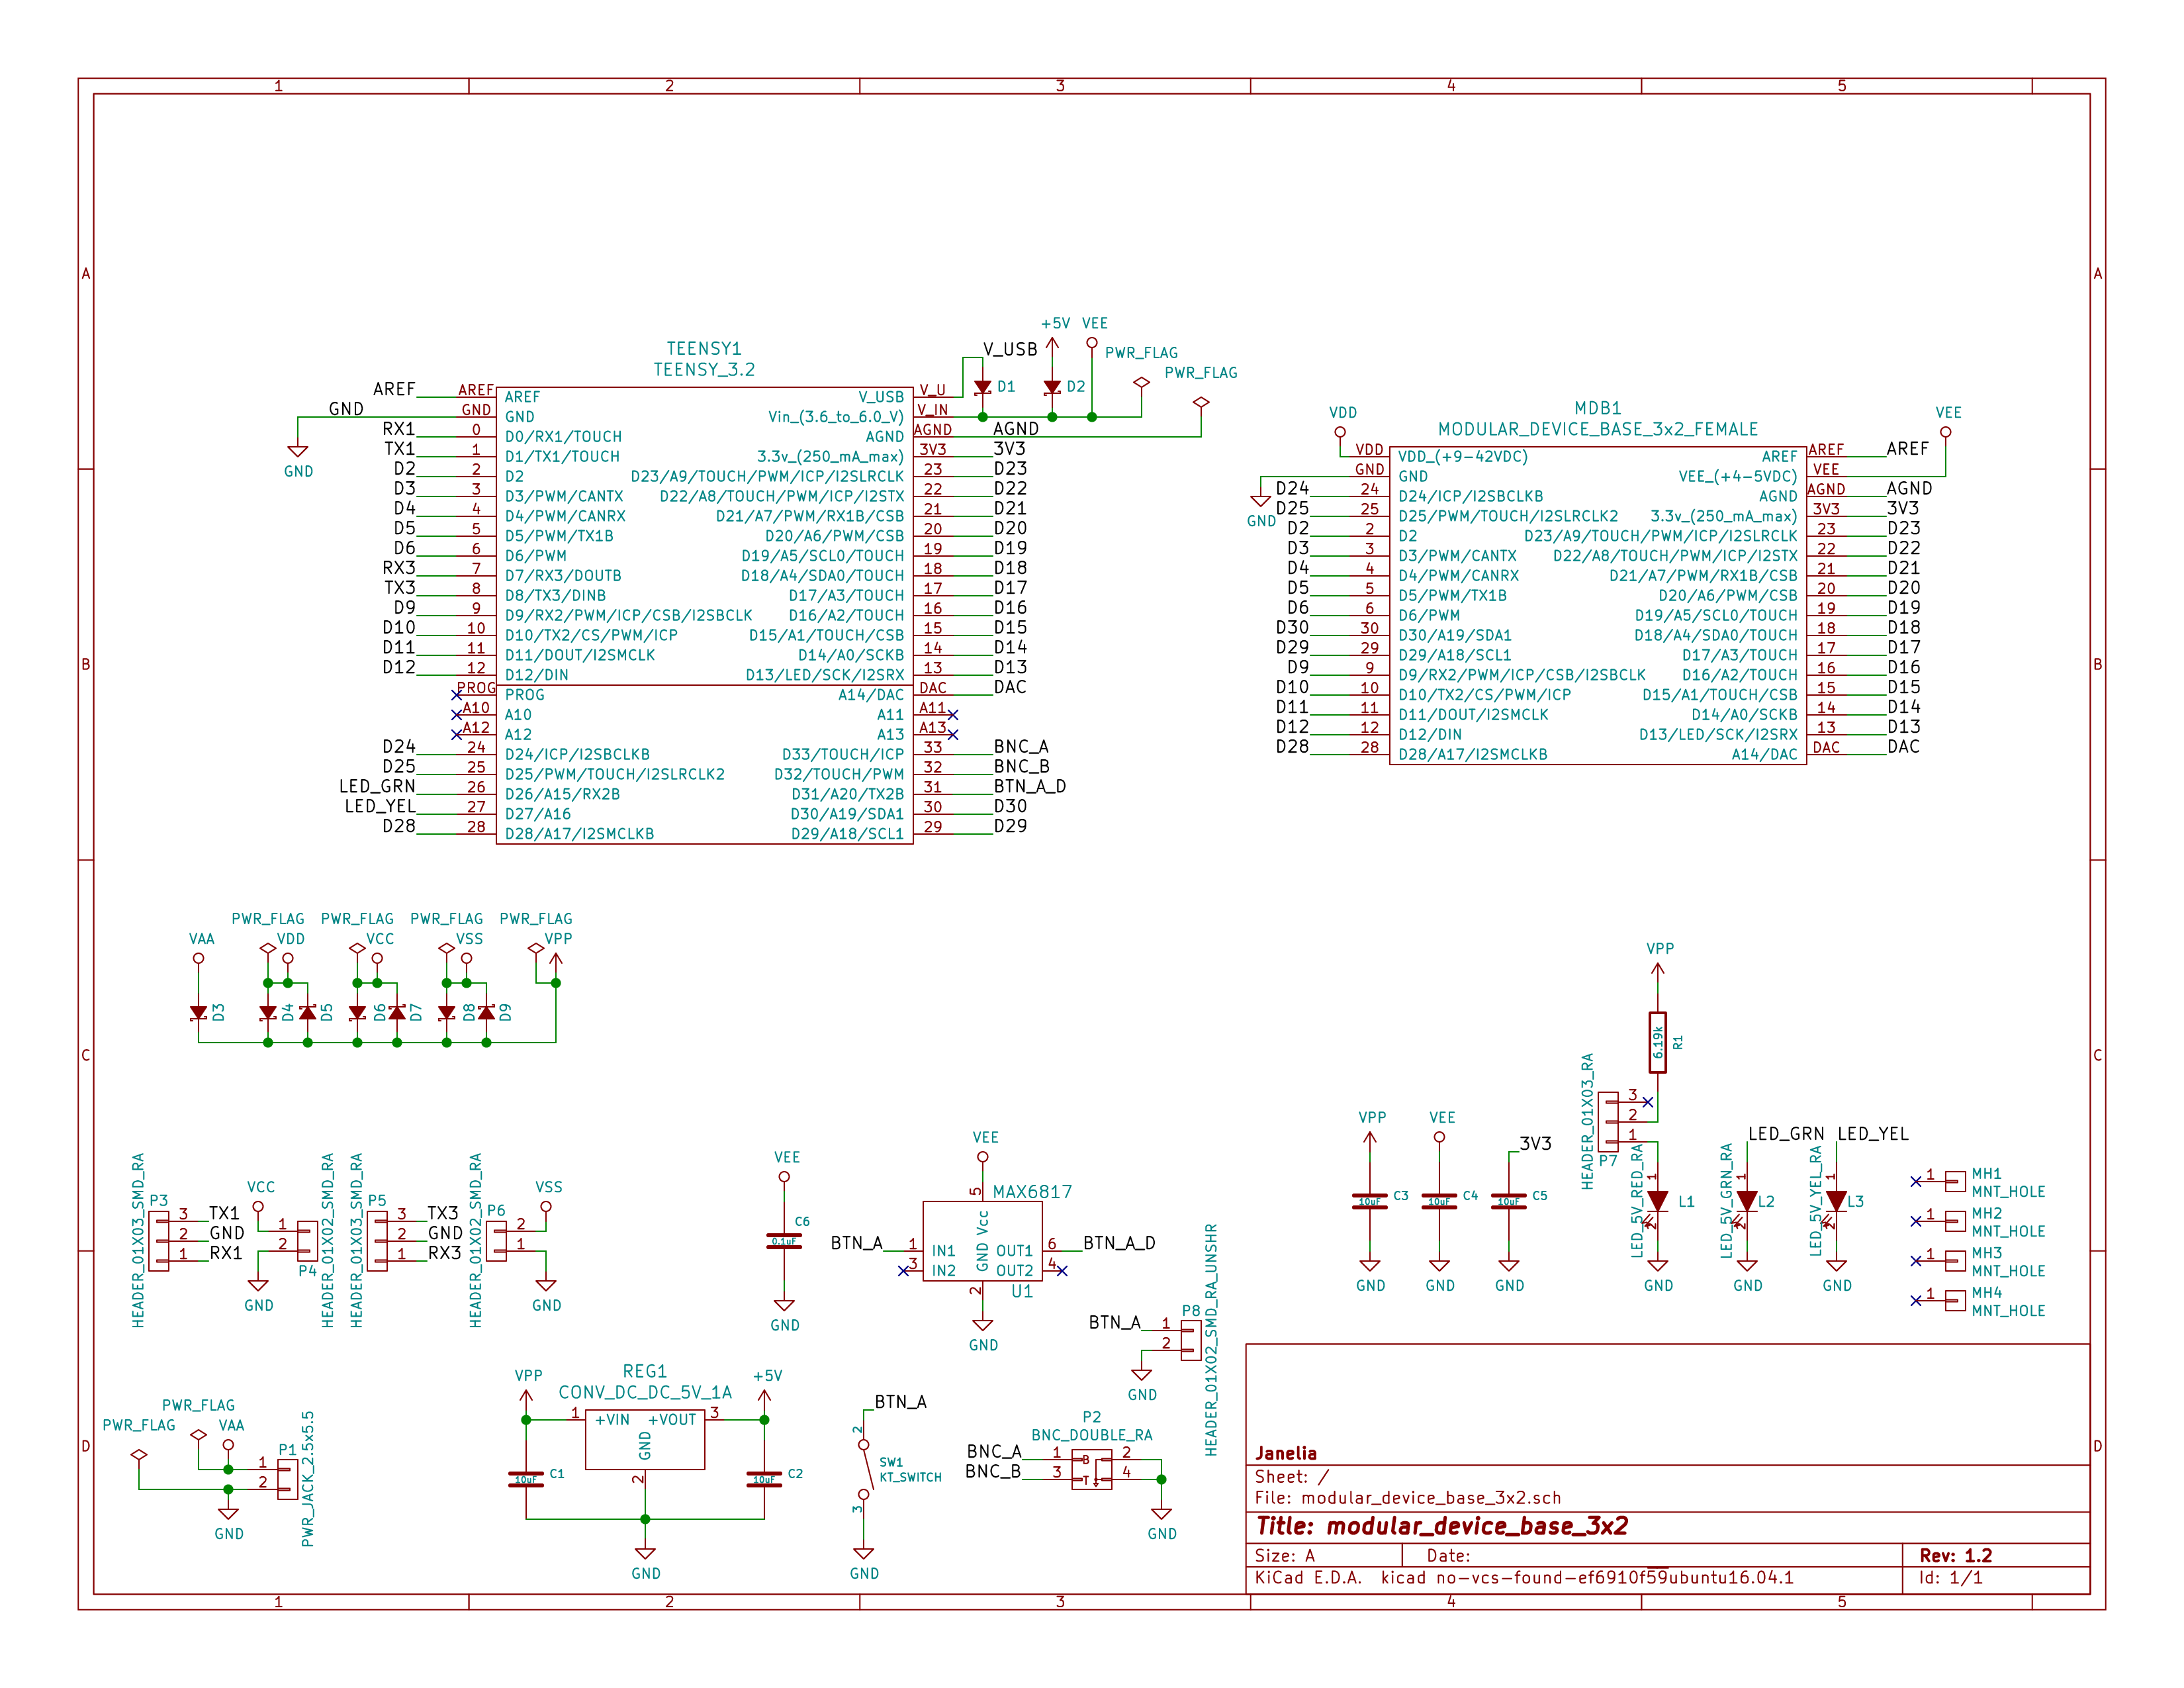
\includegraphics[width=.9\linewidth]{./schematic/images/schematic00.png}
\end{center}


\section{Gerbers}
\label{sec:orge85ae1a}

Save gerbers zip file and send to your favorite PCB manufacturer for
fabrication.

\href{./gerbers/modular\_device\_base\_3x2\_v1.2.zip}{modular\_device\_base\_3x2\_v1.2.zip}


\begin{center}
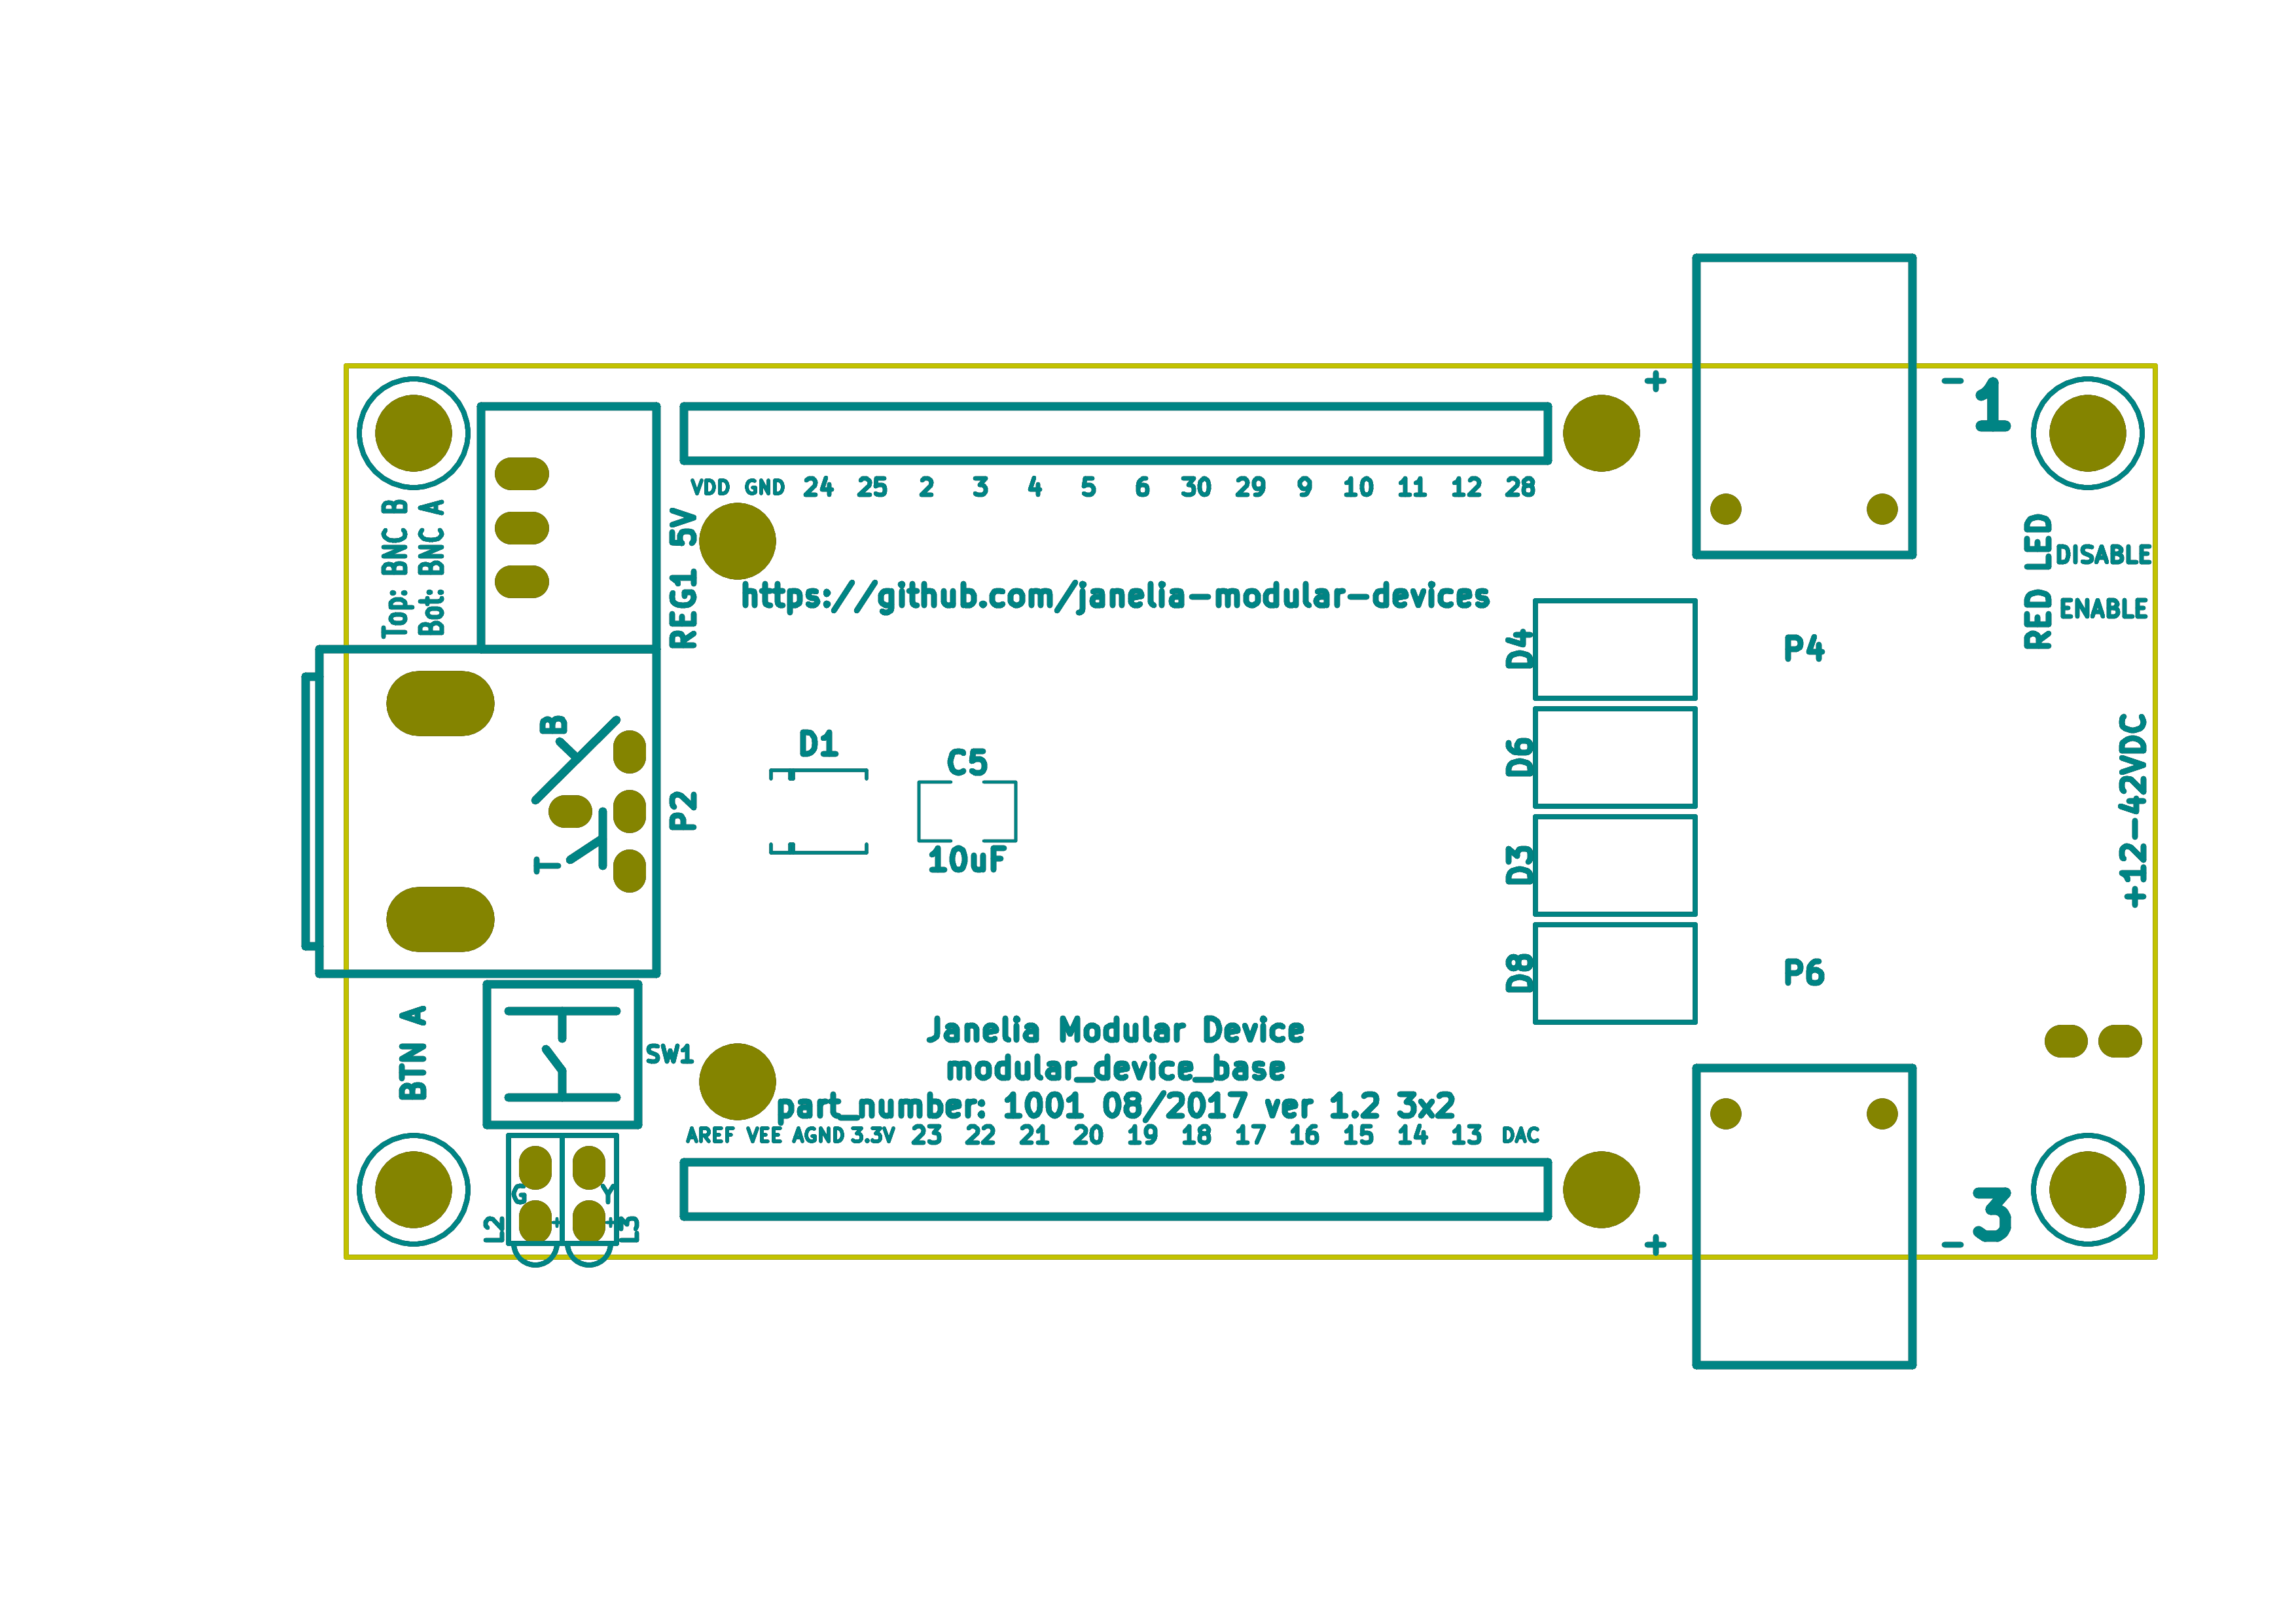
\includegraphics[width=.9\linewidth]{./gerbers/images/gerbers00.png}
\end{center}

\begin{center}
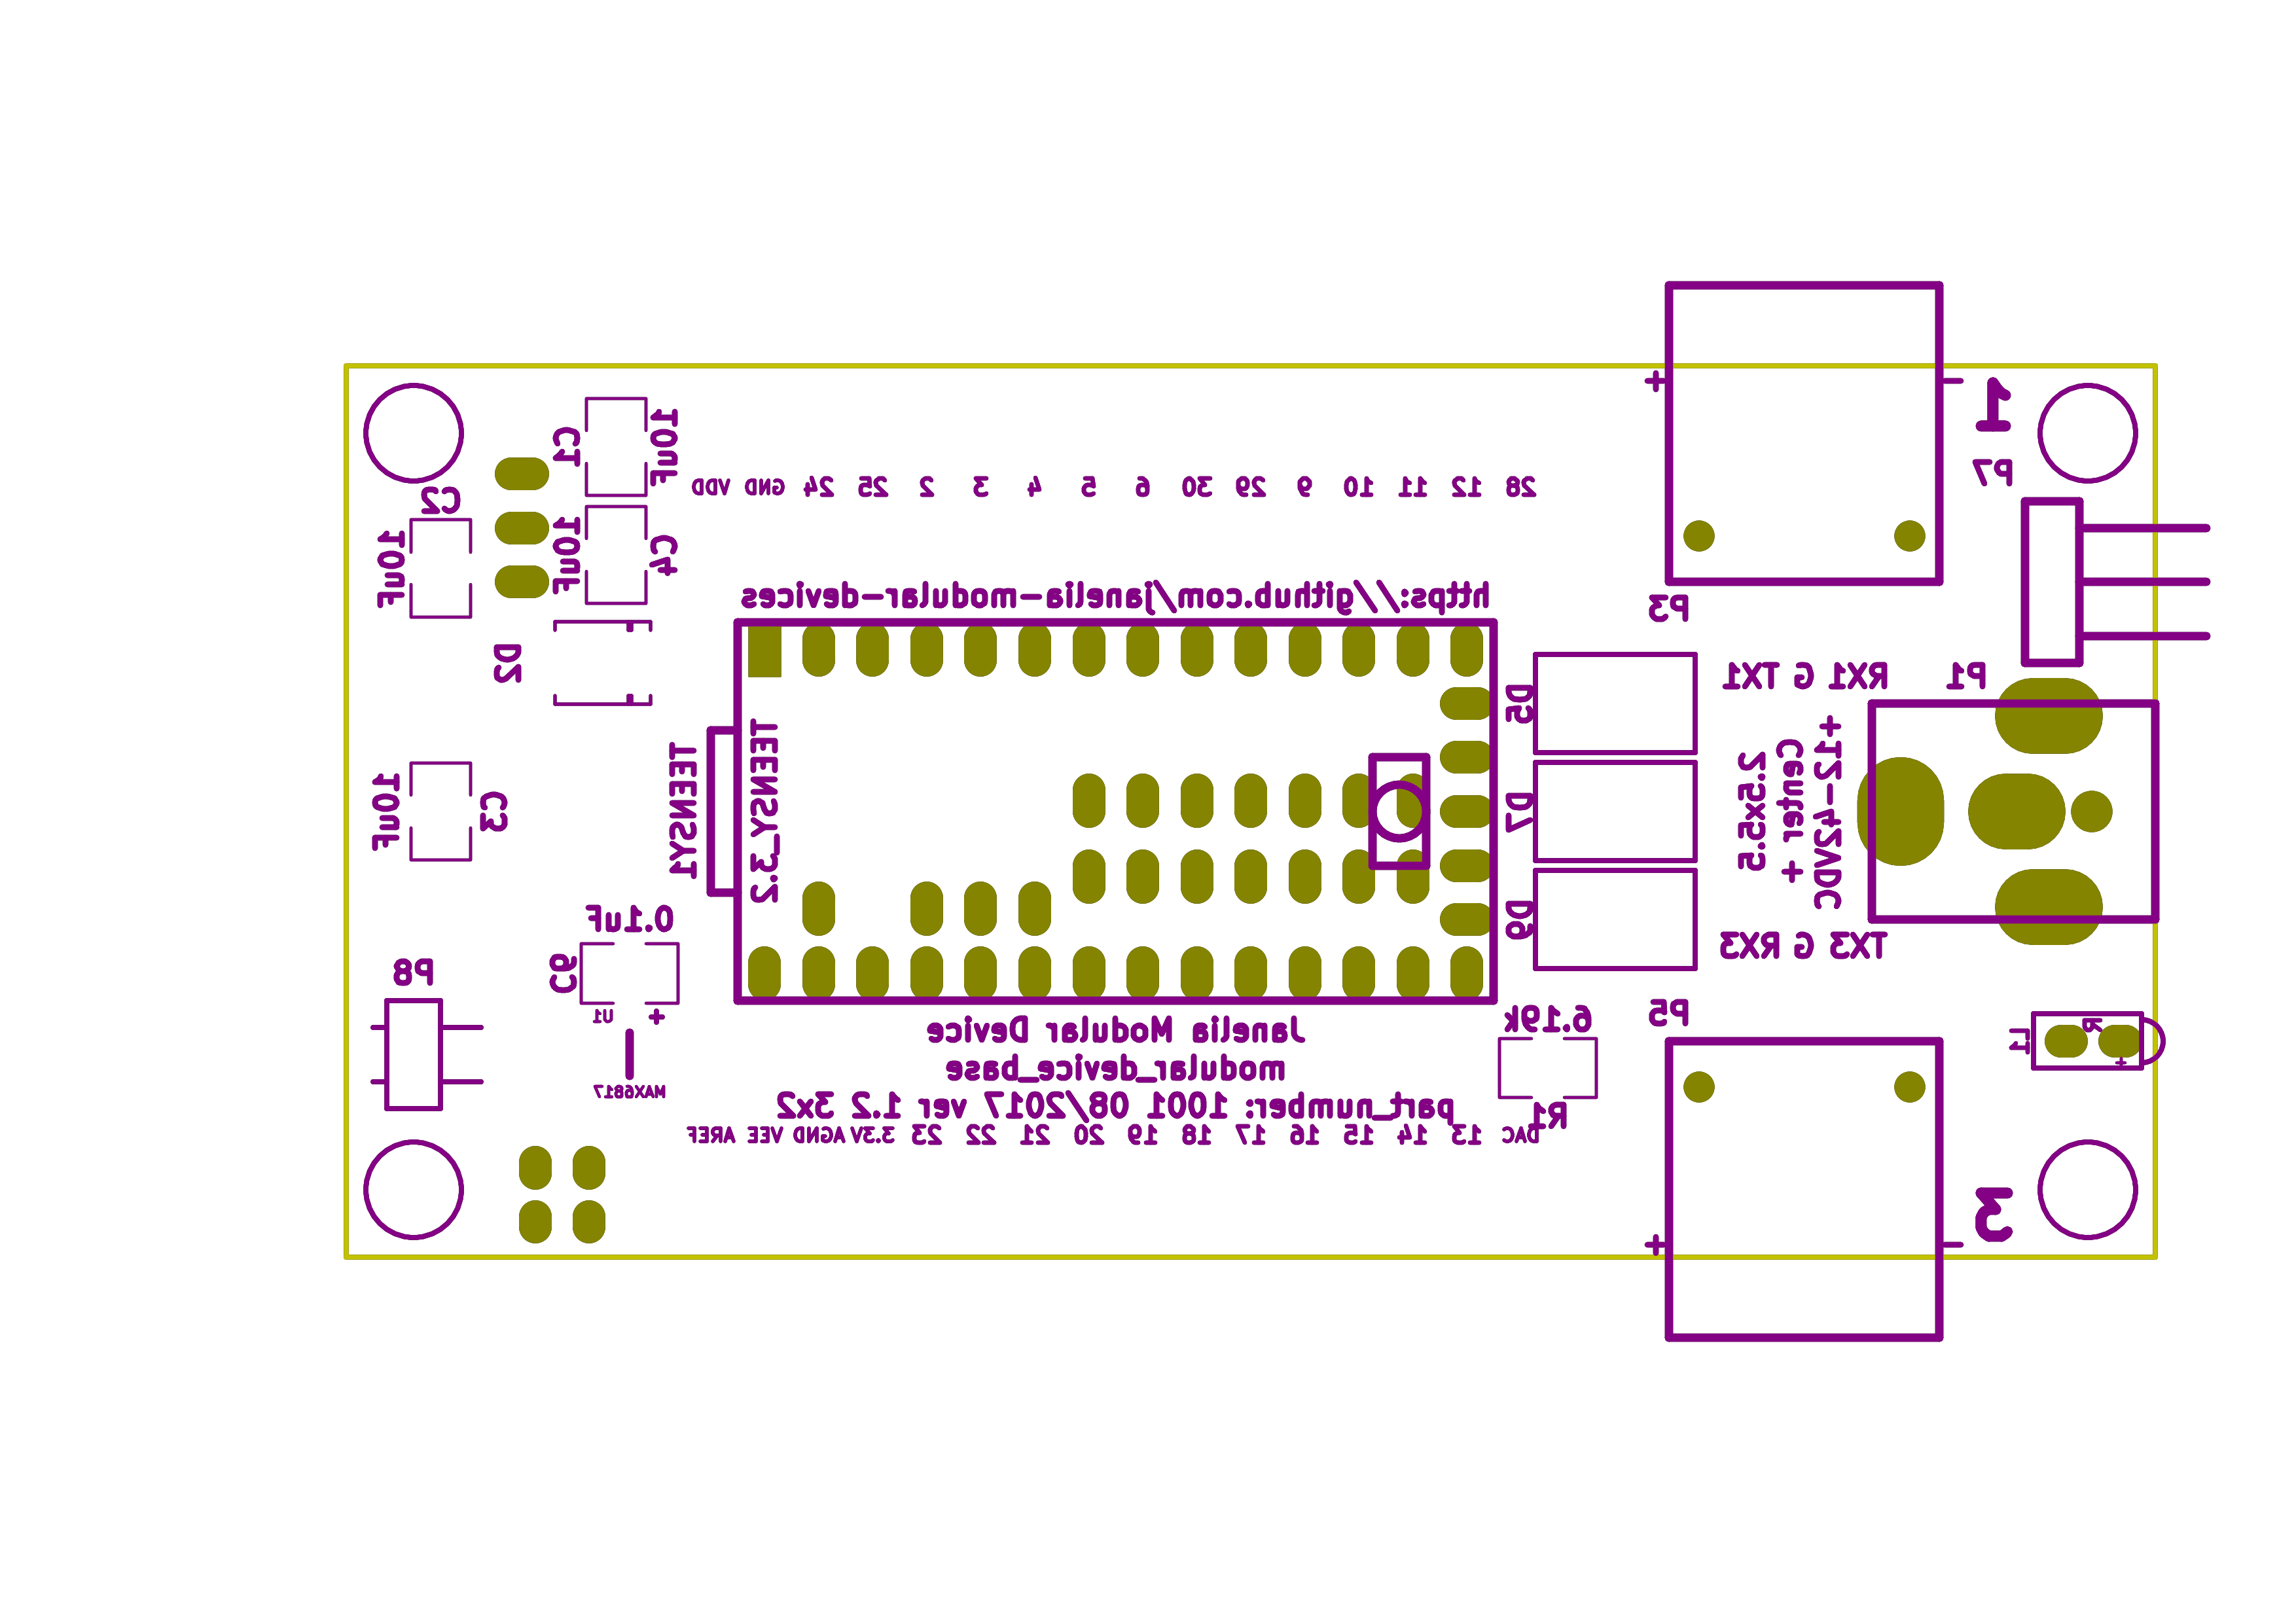
\includegraphics[width=.9\linewidth]{./gerbers/images/gerbers01.png}
\end{center}


\section{Bill of Materials}
\label{sec:orgf85580f}

./bom/bom\_pcb\_add.csv
./bom/bom\_pcb.csv
./bom/digikey\_order.csv
./bom/digikey\_order\_pcb\_add.csv
./bom/digikey\_order\_pcb.csv
\end{document}
